\documentclass{article}\usepackage[]{graphicx}\usepackage[]{xcolor}
% maxwidth is the original width if it is less than linewidth
% otherwise use linewidth (to make sure the graphics do not exceed the margin)
\makeatletter
\def\maxwidth{ %
  \ifdim\Gin@nat@width>\linewidth
    \linewidth
  \else
    \Gin@nat@width
  \fi
}
\makeatother

\definecolor{fgcolor}{rgb}{0.345, 0.345, 0.345}
\newcommand{\hlnum}[1]{\textcolor[rgb]{0.686,0.059,0.569}{#1}}%
\newcommand{\hlsng}[1]{\textcolor[rgb]{0.192,0.494,0.8}{#1}}%
\newcommand{\hlcom}[1]{\textcolor[rgb]{0.678,0.584,0.686}{\textit{#1}}}%
\newcommand{\hlopt}[1]{\textcolor[rgb]{0,0,0}{#1}}%
\newcommand{\hldef}[1]{\textcolor[rgb]{0.345,0.345,0.345}{#1}}%
\newcommand{\hlkwa}[1]{\textcolor[rgb]{0.161,0.373,0.58}{\textbf{#1}}}%
\newcommand{\hlkwb}[1]{\textcolor[rgb]{0.69,0.353,0.396}{#1}}%
\newcommand{\hlkwc}[1]{\textcolor[rgb]{0.333,0.667,0.333}{#1}}%
\newcommand{\hlkwd}[1]{\textcolor[rgb]{0.737,0.353,0.396}{\textbf{#1}}}%
\let\hlipl\hlkwb

\usepackage{framed}
\makeatletter
\newenvironment{kframe}{%
 \def\at@end@of@kframe{}%
 \ifinner\ifhmode%
  \def\at@end@of@kframe{\end{minipage}}%
  \begin{minipage}{\columnwidth}%
 \fi\fi%
 \def\FrameCommand##1{\hskip\@totalleftmargin \hskip-\fboxsep
 \colorbox{shadecolor}{##1}\hskip-\fboxsep
     % There is no \\@totalrightmargin, so:
     \hskip-\linewidth \hskip-\@totalleftmargin \hskip\columnwidth}%
 \MakeFramed {\advance\hsize-\width
   \@totalleftmargin\z@ \linewidth\hsize
   \@setminipage}}%
 {\par\unskip\endMakeFramed%
 \at@end@of@kframe}
\makeatother

\definecolor{shadecolor}{rgb}{.97, .97, .97}
\definecolor{messagecolor}{rgb}{0, 0, 0}
\definecolor{warningcolor}{rgb}{1, 0, 1}
\definecolor{errorcolor}{rgb}{1, 0, 0}
\newenvironment{knitrout}{}{} % an empty environment to be redefined in TeX

\usepackage{alltt}
\usepackage{amsmath} %This allows me to use the align functionality.
                     %If you find yourself trying to replicate
                     %something you found online, ensure you're
                     %loading the necessary packages!
\usepackage{amsfonts}%Math font
\usepackage{graphicx}%For including graphics
\usepackage{hyperref}%For Hyperlinks
\usepackage[shortlabels]{enumitem}% For enumerated lists with labels specified
                                  % We had to run tlmgr_install("enumitem") in R
\hypersetup{colorlinks = true,citecolor=black} %set citations to have black (not green) color
\usepackage{natbib}        %For the bibliography
\setlength{\bibsep}{0pt plus 0.3ex}
\bibliographystyle{apalike}%For the bibliography
\usepackage[margin=0.50in]{geometry}
\usepackage{float}
\usepackage{multicol}

%fix for figures
\usepackage{caption}
\newenvironment{Figure}
  {\par\medskip\noindent\minipage{\linewidth}}
  {\endminipage\par\medskip}
\IfFileExists{upquote.sty}{\usepackage{upquote}}{}
\begin{document}

\vspace{-1in}
\title{Lab 10 -- MATH 240 -- Computational Statistics}

\author{
  Michael Boateng \\
  Math Department  \\
  {\tt mboateng@colgate.edu}
}

\date{}

\maketitle

\begin{multicols}{2}
\begin{abstract}
According to Gallup polls, a doubling in the sample size for polls from 1000 to 2000, results in decreasing the margin of error by two percentage points. In this lab, we test this inference by first conducting a basic simulation of random binomial distribution, calculating its margin of error, and then doing same for double the sample size. Then, using data from the Gallup survey we perform resampling to approximate $\hat{p}$. Finally, we calculate the margin of error for multiple sample sizes (\texttt{n}) and probabilities (\texttt{p}). We find that the margin of error depends not only on sample size but also \texttt{p}. 
\end{abstract}

\noindent \textbf{Keywords:} resampling; simulation; distribution; point estimate

\section{Introduction}
Gallup polls in \emph{"How Are Polls Conducted?"}, claimed that with an initial sample size of carefully selected adults of 1000, the margin of error of the results obtained from such a sample is likely to be within $\pm 4 \%$. They then followed that doubling the sample size leads to a two percentage point decrease in the margin of error. We aim to test how true this assertion from Gallup polls is. 

As an example data and frame of reference, we'll use the February 3-16, 2025 poll of 1004, adults living in all 50 U.S states and D.C.. In this poll 39\% of respondents were satisfied with the position of the U.S in the world, 59\% were dissatisfied (and 2\% of no opinion).

We begin our test by making simulations of the Gallup survey and then making estimates of the margin of error from these simulations. We then calculate the true margin of error on multiple samples with different sizes and sampling distributions to effectively know how well sample size affect margin of error values. 
 
\section{Basic Simulation}
Given that the Gallup poll reported 39\% satisfaction, we take this to be our probability of success and conduct a simulation study. Using \texttt{rbinom()}, we generate 10k polls of the same sample size (\texttt{n} = 1004). We see the the distribution of this sample in figure \ref{sample.hist}

% first figure for sample size of 1004
\begin{Figure}
\begin{centering}
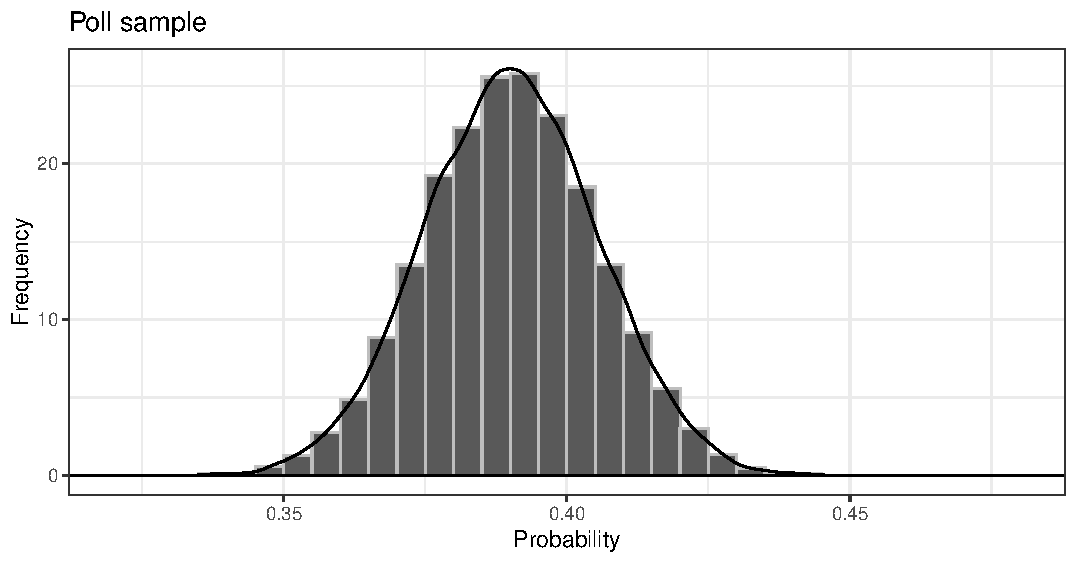
\includegraphics[width=1\columnwidth]{plots/Rplot1.pdf}
\end{centering}
\captionof{figure}{Simulation of Gallup Poll with $n = 1004$} \label{sample.hist}
\end{Figure}

From this sample, we estimate the margin of error by halving the range of the middle 95\% of the data. We find the value to be 3.03\%, which is less than the estimated 4\% from Gallup. Next we, double our sample size to obtain the distribution in figure \ref{sample2.hist}. The margin of error for this sample was 2.1\%, which is close to Gallup's reported value of 2\%. In both figure \ref{sample.hist} and \ref{sample2.hist}, we see the the data are centered around are true probability value and are also normally distributed.

% figure for double the sample size 
\begin{Figure}
\begin{centering}
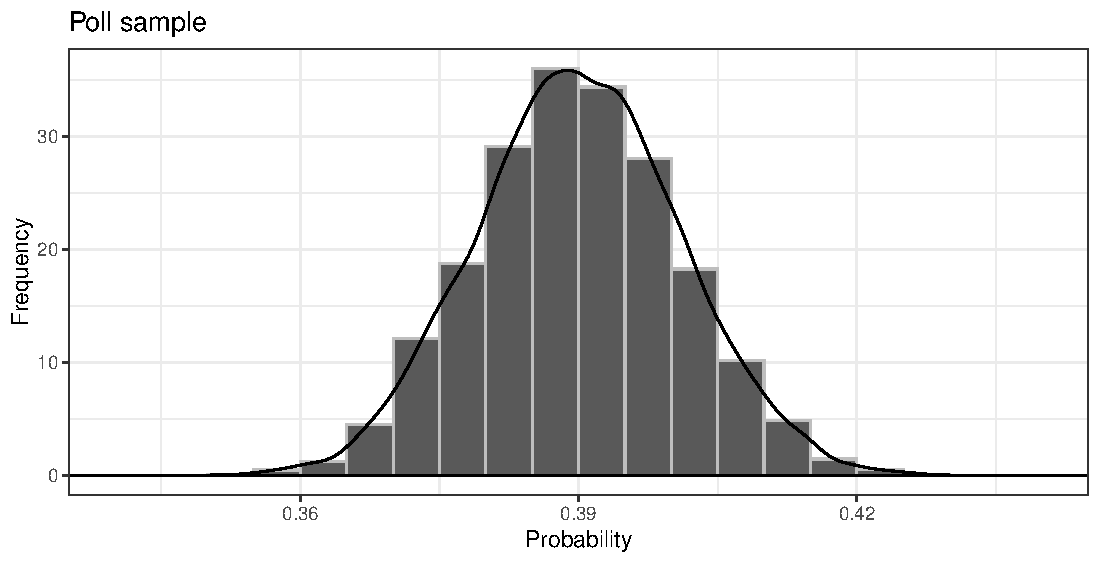
\includegraphics[width=1\columnwidth]{plots/Rplot2.pdf}
\end{centering}
\captionof{figure}{Simulation of Gallup Poll with $n = 2008$} \label{sample2.hist}
\end{Figure}

\section{Resampling}
During our simulation, we created samples of data under the assumption that ($p = 0.39$). Another way of obtaining the value of $p$, is through resampling. In resampling, we make repeated samples of an original sample and calculate our statistic of interest with each iteration, and then after we make summaries on the particular statistic. 

We performed resampling on the Gallup data (with our statistic of interest being the mean (i.e percent "satistified")), and created a graphical summary in figure \ref{resamp.hist} below. We see that our sampling distribution is normally distributed, and also heavily centered around our true probability value ($0.39$). We calcuated the margin of error on the resampling data to be 3.07\%, which is less than Gallup's report of 4\%.

% figure for Gallup data resampling
\begin{Figure}
\begin{centering}
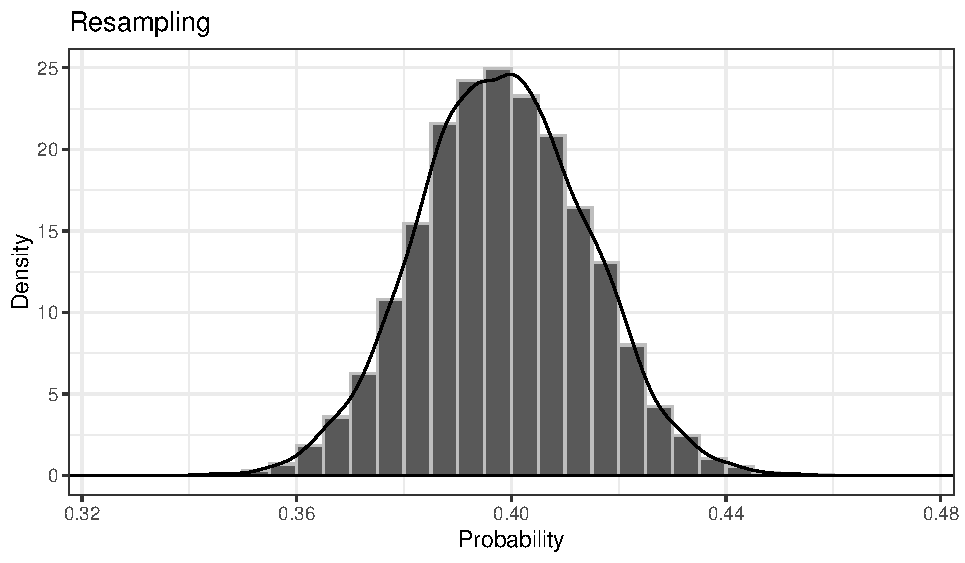
\includegraphics[width=1\columnwidth]{plots/Rplot3.pdf}
\end{centering}
\captionof{figure}{Resampling Distribution} \label{resamp.hist}
\end{Figure}

\section{Simulation over $n$ and $p$}
We now consider the effect of not just sample size but also the probability of success on margin of error values.  

For $n$ in $\{100, 110, 120, ... ,3000\}$ and $p$ in $\{0.01, 0.02, ..., 0.99\}$, we perform 10k simulations and each time calculating and storing the estimated margin of error. The simulations are summarized in figure \ref{sim.raster} below.

% figure for simulation over n and p
\begin{Figure}
\begin{centering}
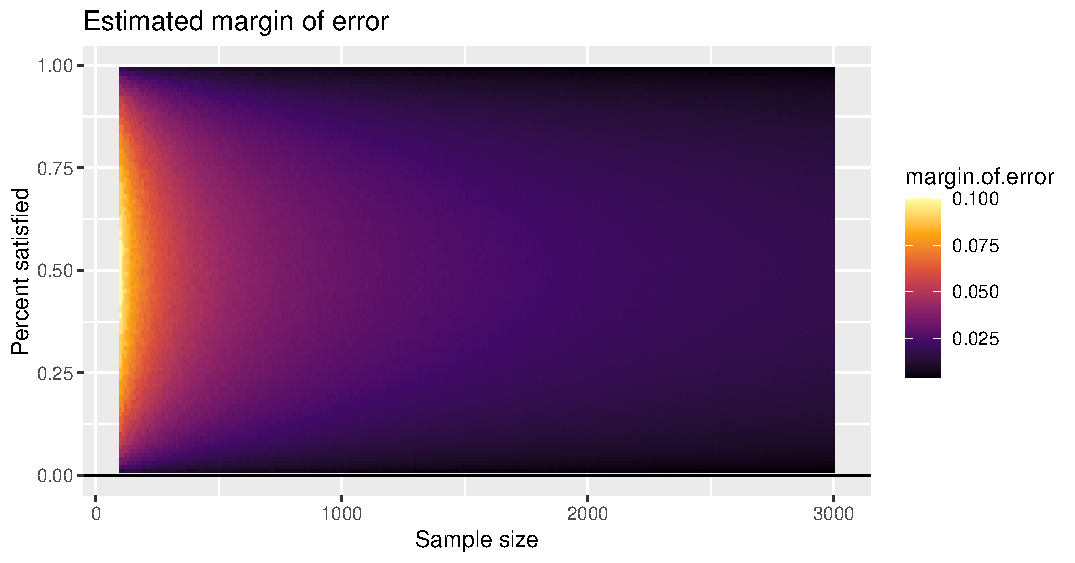
\includegraphics[width=1\columnwidth]{plots/Rplot4.pdf}
\end{centering}
\captionof{figure}{Margin of error as a function of $n$ and $p$} \label{sim.raster}
\end{Figure}

\subsection{Actual Margin of Error Calcuation}
Previously, we had estimated the margin of error by halving the range of the middle 95\%. However using Wilson's estimate we can find the actual margin of error of the data.

We computer the margin of error using the Wilson formula for $n$ in $\{100, 110, 120, ... ,2000\}$ and $p$ in $\{0.01, 0.02, ..., 0.99\}$. Results summarized in figure \ref{wilson.raster}.

% wilson's estimate for simulation over n and p
\begin{Figure}
\begin{centering}
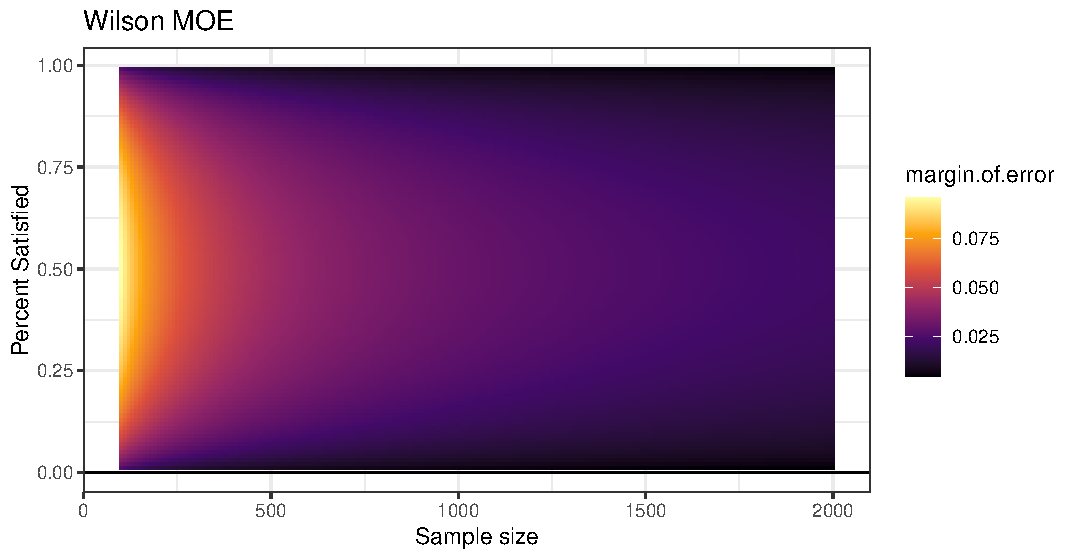
\includegraphics[width=1\columnwidth]{plots/Rplot5.pdf}
\end{centering}
\captionof{figure}{Margin of error as a function of $n$ and $p$ (wilson's estimate)} \label{wilson.raster}
\end{Figure}



\section{Discussion}
While Gallup's report of how a double in sample size decreases the margin pf error is true to some extent, it does not reflect how the value of $p$ can also influence the change in margin of error. Regardless of sample size, we see in figure \ref{sim.raster} and \ref{wilson.raster}, is smallest as $p$ takes a value close to the extremes (0 or 1). However, looking at the same graph we see that margin of error, is greater for smaller for larger sample sizes that smaller one for non-extreme values of $p$.

This suggests that the actual story is not as simple Gallup made it out to be. For extreme population proportion values, doubling our sample data will not yield such a change in margin of error.

%%%%%%%%%%%%%%%%%%%%%%%%%%%%%%%%%%%%%%%%%%%%%%%%%%%%%%%%%%%%%%%%%%%%%%%%%%%%%%%%
% Bibliography
%%%%%%%%%%%%%%%%%%%%%%%%%%%%%%%%%%%%%%%%%%%%%%%%%%%%%%%%%%%%%%%%%%%%%%%%%%%%%%%%
\vspace{2em}


\begin{tiny}
\bibliography{bib}
\end{tiny}
\end{multicols}

%%%%%%%%%%%%%%%%%%%%%%%%%%%%%%%%%%%%%%%%%%%%%%%%%%%%%%%%%%%%%%%%%%%%%%%%%%%%%%%%
% Appendix
%%%%%%%%%%%%%%%%%%%%%%%%%%%%%%%%%%%%%%%%%%%%%%%%%%%%%%%%%%%%%%%%%%%%%%%

\end{document}
